% Options for packages loaded elsewhere
\PassOptionsToPackage{unicode}{hyperref}
\PassOptionsToPackage{hyphens}{url}
%
\documentclass[
]{book}
\usepackage{lmodern}
\usepackage{amssymb,amsmath}
\usepackage{ifxetex,ifluatex}
\ifnum 0\ifxetex 1\fi\ifluatex 1\fi=0 % if pdftex
  \usepackage[T1]{fontenc}
  \usepackage[utf8]{inputenc}
  \usepackage{textcomp} % provide euro and other symbols
\else % if luatex or xetex
  \usepackage{unicode-math}
  \defaultfontfeatures{Scale=MatchLowercase}
  \defaultfontfeatures[\rmfamily]{Ligatures=TeX,Scale=1}
\fi
% Use upquote if available, for straight quotes in verbatim environments
\IfFileExists{upquote.sty}{\usepackage{upquote}}{}
\IfFileExists{microtype.sty}{% use microtype if available
  \usepackage[]{microtype}
  \UseMicrotypeSet[protrusion]{basicmath} % disable protrusion for tt fonts
}{}
\makeatletter
\@ifundefined{KOMAClassName}{% if non-KOMA class
  \IfFileExists{parskip.sty}{%
    \usepackage{parskip}
  }{% else
    \setlength{\parindent}{0pt}
    \setlength{\parskip}{6pt plus 2pt minus 1pt}}
}{% if KOMA class
  \KOMAoptions{parskip=half}}
\makeatother
\usepackage{xcolor}
\IfFileExists{xurl.sty}{\usepackage{xurl}}{} % add URL line breaks if available
\IfFileExists{bookmark.sty}{\usepackage{bookmark}}{\usepackage{hyperref}}
\hypersetup{
  pdftitle={O czym śpiewają Holendrzy?},
  pdfauthor={Jacek Pardyak},
  hidelinks,
  pdfcreator={LaTeX via pandoc}}
\urlstyle{same} % disable monospaced font for URLs
\usepackage{longtable,booktabs}
% Correct order of tables after \paragraph or \subparagraph
\usepackage{etoolbox}
\makeatletter
\patchcmd\longtable{\par}{\if@noskipsec\mbox{}\fi\par}{}{}
\makeatother
% Allow footnotes in longtable head/foot
\IfFileExists{footnotehyper.sty}{\usepackage{footnotehyper}}{\usepackage{footnote}}
\makesavenoteenv{longtable}
\usepackage{graphicx}
\makeatletter
\def\maxwidth{\ifdim\Gin@nat@width>\linewidth\linewidth\else\Gin@nat@width\fi}
\def\maxheight{\ifdim\Gin@nat@height>\textheight\textheight\else\Gin@nat@height\fi}
\makeatother
% Scale images if necessary, so that they will not overflow the page
% margins by default, and it is still possible to overwrite the defaults
% using explicit options in \includegraphics[width, height, ...]{}
\setkeys{Gin}{width=\maxwidth,height=\maxheight,keepaspectratio}
% Set default figure placement to htbp
\makeatletter
\def\fps@figure{htbp}
\makeatother
\setlength{\emergencystretch}{3em} % prevent overfull lines
\providecommand{\tightlist}{%
  \setlength{\itemsep}{0pt}\setlength{\parskip}{0pt}}
\setcounter{secnumdepth}{5}
% new for polish
\usepackage{polski}
\usepackage[polish]{babel}
%\usepackage[utf8]{inputenc}

% ------------
\usepackage{booktabs}
\usepackage{amsthm}
\makeatletter
\def\thm@space@setup{%
  \thm@preskip=8pt plus 2pt minus 4pt
  \thm@postskip=\thm@preskip
}
% ------------
% new for columns
\newenvironment{columns}[1][]{}{}

\newenvironment{column}[1]{\begin{minipage}{#1}\ignorespaces}{%
\end{minipage}
\ifhmode\unskip\fi
\aftergroup\useignorespacesandallpars}

\def\useignorespacesandallpars#1\ignorespaces\fi{%
#1\fi\ignorespacesandallpars}

\makeatletter
\def\ignorespacesandallpars{%
  \@ifnextchar\par
    {\expandafter\ignorespacesandallpars\@gobble}%
    {}%
}
\makeatother
\usepackage[]{natbib}
\bibliographystyle{apalike}

\title{O czym śpiewają Holendrzy?}
\author{Jacek Pardyak}
\date{2020-04-23}

\begin{document}
\maketitle

{
\setcounter{tocdepth}{1}
\tableofcontents
}
\hypertarget{wstux119p}{%
\chapter{Wstęp}\label{wstux119p}}

Remember each Rmd file contains one and only one chapter, and a chapter is defined by the first-level heading \texttt{\#}.

To compile this example to PDF, you need XeLaTeX. You are recommended to install TinyTeX (which includes XeLaTeX): \url{https://yihui.name/tinytex/}.

\hypertarget{lata-1970-1979}{%
\chapter{Lata 1970-1979}\label{lata-1970-1979}}

\hypertarget{lata-1980-1989}{%
\chapter{Lata 1980-1989}\label{lata-1980-1989}}

\hypertarget{Een-beetje-verliefd}{%
\section{\texorpdfstring{Een beetje verliefd, \emph{André Hazes}}{Een beetje verliefd, André Hazes}}\label{Een-beetje-verliefd}}

\begin{column}{0.36\textwidth}

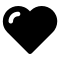
\includegraphics{./images/Een-beetje-verliefd}

\end{column}

\begin{column}{0.04\textwidth}

~

\end{column}

\begin{column}{0.60\textwidth}

Piosenka \textbf{Een beetje verliefd} \citep{Een-beetje-verliefd} \emph{Trochę zakochany} .

\end{column}

\vfill

\begin{column}{0.48\textwidth}

In een discotheek, zat ik van de week\\
En ik voelde mij daar zo alleen\\
't Was er warm en druk, ik zat naast een lege kruk\\
Ik verlangde zo naar jou hier aan m'n zij

\end{column}

\begin{column}{0.04\textwidth}

~

\end{column}

\begin{column}{0.48\textwidth}

W jakiejś dyskotece byłem na tygodniu\\
I czułem się tam bardzo samotny\\
Było tam gorąco i tłoczno, siedziałem przy pustym stołku\\
Tak pragnąłem cię tutaj przy moim boku

\end{column}

\vfill

\begin{column}{0.48\textwidth}

Ja, ik denk nog steeds hoe het was geweest\\
Toen je naast me zat hier aan de bar\\
Ik vroeg: `'Drink je mee?'', dat vond jij oké\\
Toen je proostend naar me keek werd ik zo week

\end{column}

\begin{column}{0.04\textwidth}

~

\end{column}

\begin{column}{0.48\textwidth}

Tak, wciąż się zastanawiam, jak to było\\
Gdy się do mnie przysiadłaś przy barze\\
Spytałem: `'Napijesz się ze mną?'', zgodziłaś się\\
Kiedy na mnie spojrzałaś przy toaście, stałem się taki miękki

\end{column}

\vfill

\begin{column}{0.48\textwidth}

\emph{Een beetje verliefd, ik dacht een beetje verliefd}\\
\emph{Als ik wist wat jij toen dacht, had ik nooit op jou gewacht}\\
\emph{Als een kind zat ik te dromen deze nacht ben jij voor mij}\\
\emph{Maar die droom ging snel voorbij}

\end{column}

\begin{column}{0.04\textwidth}

~

\end{column}

\begin{column}{0.48\textwidth}

\emph{Trochę zakochany, myślałem trochę zakochany}\\
\emph{Gdybym wiedział, co wtedy myślisz, nigdy bym na ciebie nie czekał}\\
\emph{Jak małe dziecko ciągle marzyłem, tej nocy jesteś dla mnie}\\
\emph{Ale ten sen szybko minął}

\end{column}

\vfill

\begin{column}{0.48\textwidth}

Jij stond op en zei: `'Hou m'n plaatsje vrij\\
Ik moet even weg maar ben zo terug''\\
Ach, die kruk bleef leeg tot ik in de gaten kreeg\\
Dat je wegging zonder mij, ik was nu alleen

\end{column}

\begin{column}{0.04\textwidth}

~

\end{column}

\begin{column}{0.48\textwidth}

Wstałaś i powiedziałaś: `'Zajmij mi miejsce\\
ja muszę na chwilę wyjść, ale zaraz wrócę''\\
Ach, ten stołek stał pusty, dopóki nie zauważyłem\\
Że odeszłaś beze mnie, teraz byłem sam

\end{column}

\vfill

\begin{quote}
\textbf{Weet je wat, ik ben er zat van.} Wiesz co, mam tego dosyć.\\
\textbf{Ik verlang ernaar met je alleen te zijn.} Pragnę być z tobą sam.\\
\textbf{Ik heb de wet aan m'n zij(-de).} Prawo mam po swojej stronie.\\
\textbf{Dat vind ik erg leuk.} To mi się bardzo podoba.\\
\textbf{We zitten te praten.} Gadamy sobie.\\
\textbf{Ik krijg dit in de gaten.} Zdaję sobie sprawę z tego
\end{quote}

\hypertarget{lata-1990---1999}{%
\chapter{Lata 1990 - 1999}\label{lata-1990---1999}}

\hypertarget{Leef}{%
\section{\texorpdfstring{Leef, \emph{Han van Eijk}}{Leef, Han van Eijk}}\label{Leef}}

\begin{column}{0.36\textwidth}

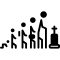
\includegraphics{./images/Leef}

\end{column}

\begin{column}{0.04\textwidth}

~

\end{column}

\begin{column}{0.60\textwidth}

Piosenka \textbf{Leef} \citep{Leef} \emph{Żyj} stała się hitem list przebojów po tym została użyta w pierwszej w Holandii edycji Big Brother.

\end{column}

\vfill

\begin{column}{0.48\textwidth}

Niemand hoeft alleen maar goed of slecht te zijn\\
Niemand is alleen maar zwart of wit\\
Iedereen is anders, anders dan je verwacht

\end{column}

\begin{column}{0.04\textwidth}

~

\end{column}

\begin{column}{0.48\textwidth}

Nikt nie musi być albo dobry albo zły\\
Nikt nie jest albo biały albo czarny\\
Każdy jest inny, inny niż się spodziewasz

\end{column}

\vfill

\begin{column}{0.48\textwidth}

Niemand die alleen maar haat of liefde voelt\\
We zijn allemaal een mens van vlees en bloed\\
En we kunnen niet perfect zijn want niemand weet hoe dat moet

\end{column}

\begin{column}{0.04\textwidth}

~

\end{column}

\begin{column}{0.48\textwidth}

Niemand die alleen maar haat of liefde voelt\\
We zijn allemaal een mens van vlees en bloed\\
En we kunnen niet perfect zijn want niemand weet hoe dat moet

\end{column}

\vfill

\begin{column}{0.48\textwidth}

\_ Leef, met je eigen talent\_\\
\_ Iedereen is mooi, als bent wie je bent\_\\
\_ Leef, met jezelf en elkaar\_\\
\_ Iedereen is blij met dat ene gebaar\_

\end{column}

\begin{column}{0.04\textwidth}

~

\end{column}

\begin{column}{0.48\textwidth}

\_ Żyj z własnym talentem\_\\
\_ Iedereen is mooi, als bent wie je bent\_\\
\_ Leef, met jezelf en elkaar\_\\
\_ Iedereen is blij met dat ene gebaar\_

\end{column}

\vfill

\begin{column}{0.48\textwidth}

Niemand kan alleen maar mooi of lelijk zijn\\
Niemand heeft de waarheid vol in beeld\\
Maar het voordeel van de twijfel maakt ons minder verdeeld\\
We zoeken de verschillen, waar we bruggen moeten bouwen

\end{column}

\begin{column}{0.04\textwidth}

~

\end{column}

\begin{column}{0.48\textwidth}

Nikt nie może być tylko piękny albo brzydki\\
Niemand heeft de waarheid vol in beeld\\
Maar het voordeel van de twijfel maakt ons minder verdeeld\\
We zoeken de verschillen, waar we bruggen moeten bouwen

\end{column}

\vfill

\begin{column}{0.48\textwidth}

En we plakken etiketten op het hart van iedereen\\
Maar het leven is geen leven als geen mens van je wil houden\\
Dus we moeten bruggen bouwen over alle kloven heen\\
Niemand hoeft alleen maar goed of slecht te zijn

\end{column}

\begin{column}{0.04\textwidth}

~

\end{column}

\begin{column}{0.48\textwidth}

I umieszczamy etykiety na sercu każdego\\
Ale życie nie jest życiem, jeśli nikt nie chce cię kochać\\
Musimy więc budować mosty nad wszystkimi lukami\\
Niemand hoeft alleen maar goed of slecht te zijn

\end{column}

\vfill

\begin{quote}
\textbf{Je hoeft niet bang te zijn om fouten te maken.} Nie musisz bać się popełniać błędów.\\
\textbf{Ik zeg het alleen maar!} Po prostu to mówię!\\
\textbf{Gele gans zelf.} Zażółć gęślą jaźń.
\end{quote}

\hypertarget{Het-is-een-nacht}{%
\section{\texorpdfstring{Het is een nacht, \emph{Guus Meeuwis}}{Het is een nacht, Guus Meeuwis}}\label{Het-is-een-nacht}}

\begin{column}{0.36\textwidth}

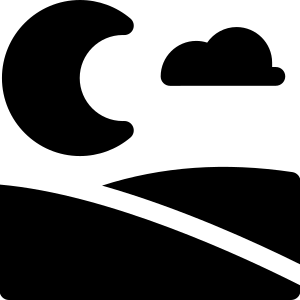
\includegraphics{./images/Het-is-een-nacht}

\end{column}

\begin{column}{0.04\textwidth}

~

\end{column}

\begin{column}{0.60\textwidth}

Piosenka \textbf{Het is een nacht} \citep{Het-is-een-nacht} \emph{To jest taka noc} powstała po romantycznym weekendzie, jaki spędził autor ze swoją dziewczyną Valérie Gregoire w Brugii.

\end{column}

\vfill

\begin{column}{0.48\textwidth}

Je vraagt of ik zin heb in een sigaret\\
Het is twee uur 's nachts\\
We liggen op bed\\
In een hotel in een stad\\
Waar niemand ons hoort\\
Waar niemand ons kent\\
En niemand ons stoort\\
Op de vloer ligt een lege fles wijn\\
En kledingstukken die van jou of mij kunnen zijn\\
Een schemering de radio zacht\\
En deze nacht heeft alles\\
Wat ik van een nacht verwacht

\end{column}

\begin{column}{0.04\textwidth}

~

\end{column}

\begin{column}{0.48\textwidth}

Pytasz, czy mam ochotę na papierosa\\
Jest druga w nocy\\
Jesteśmy w łóżku\\
W hotelu, w mieście\\
Gdzie nikt nas nie słyszy\\
Gdzie nikt nas nie zna\\
I nikt nam nie przeszkadza\\
Na podłodze leży pusta butelka po winie\\
I ubrania, które mogą być twoje lub moje\\
Półmrok, radio cicho gra\\
I ta noc ma wszystko\\
Czego oczekuję od nocy

\end{column}

\vfill

\begin{column}{0.48\textwidth}

\emph{Het is een nacht}\\
\emph{Die je normaal alleen in films ziet}\\
\emph{Het is een nacht}\\
\emph{Die wordt bezongen in het mooiste lied}\\
\emph{Het is een nacht}\\
\emph{Waarvan ik dacht dat ik hem nooit beleven zou}\\
\emph{Maar vannacht beleef ik hem met jou ohoh}

\end{column}

\begin{column}{0.04\textwidth}

~

\end{column}

\begin{column}{0.48\textwidth}

\emph{To jest taka noc}\\
\emph{Którą widzisz zwykle tylko w filmach}\\
\emph{To jest taka noc}\\
\emph{O której mówi najpiękniejsza piosenka}\\
\emph{To jest taka noc}\\
\emph{O której myślałem, że jej nigdy nie przeżyję}\\
\emph{A którą dziś przeżywam z tobą Ooo\ldots{}}

\end{column}

\vfill

\begin{column}{0.48\textwidth}

Ik ben nog wakker en ik staar naar het plafond\\
En ik denk aan de dag lang geleden begon\\
Het zomaar er vandoor gaan met jou\\
Niet wetend waar de reis eindigen zou\\
Nu lig ik hier in een wildvreemde stad\\
En heb net de nacht van mijn leven gehad\\
Maar helaas er komt weer licht door de ramen\\
Hoewel voor ons de wereld\\
Vannacht heeft stil gestaan

\end{column}

\begin{column}{0.04\textwidth}

~

\end{column}

\begin{column}{0.48\textwidth}

Nadal nie śpię i wpatruję się w sufit\\
I myślę o tym dniu co zaczął się tak dawno\\
Tak po prostu przemija przy tobie\\
Nie wiedząc, gdzie zakończy się ta podróż\\
Teraz leżę tutaj w zupełnie obcym mieście\\
I właśnie miałem noc swojego życia\\
Ale niestety światło znów wpada przez okna\\
Ale co tam, świat dla nas\\
Zatrzymał się dziś w nocy

\end{column}

\vfill

\begin{column}{0.48\textwidth}

Maar een lied blijft slechts bij woorden\\
Een film is in scene gezet\\
Maar deze nacht met jou\\
Is levensecht

\end{column}

\begin{column}{0.04\textwidth}

~

\end{column}

\begin{column}{0.48\textwidth}

Ale piosenka to tylko słowa\\
Film jest na scenie zagrany\\
Ale dzisiejsza noc z tobą\\
Jest prawdziwa

\end{column}

\vfill

\begin{column}{0.48\textwidth}

En vannacht beleef ik hem met jou ohoh\\
En ik hou alleen nog maar van jou ohoh\\
En ik hou alleen nog maar van jou

\end{column}

\begin{column}{0.04\textwidth}

~

\end{column}

\begin{column}{0.48\textwidth}

I dziś przeżywam ją z tobą Ooo\ldots{}\\
I kocham tylko wyłącznie ciebie Ooo\ldots{}\\
I kocham tylko wyłącznie ciebie

\end{column}

\vfill

\begin{quote}
\textbf{Je bent trouwens eigenlijk wel geweldig.} Nawiasem mówiąc, jesteś naprawdę świetny.\\
\textbf{Als ik niet Pools was, zou ik geen Pools kennen.} Gdybym nie był Polakiem, nie znałbym polskiego.\\
\textbf{Heb ik daarvoor een vergunning nodig?} Czy potrzebuję na to zezwolenie?\\
\textbf{Waar kan ik meer te weten komen over \ldots?} Gdzie mogę dowiedzieć się więcej o\ldots?\\
\textbf{Wanneer \ldots{}} Kiedy \ldots\ldots..?\\
\textbf{Ik heb zin in een borrel.} Mam ochotę na drinka.\\
\textbf{De lijn is bezet. Linia jest zajęta}\\
\textbf{Als ik meer tijd had, zou ik op je wachten.} Gdybym miał/a więcej czasu, poczekałbym na ciebie.\\
\textbf{Je moeder kan echt lekker koken.} Twoja mama naprawdę potrafi dobrze gotować.\\
\textbf{Dat is veel, he?} To dużo, prawda?\\
\textbf{Wanneer moet ik terugkomen?} Kiedy muszę wrócić?\\
\textbf{Zullen wij naar de duinen gaan?} Może pójdziemy na wydmy?
\end{quote}

\hypertarget{lata-2000---2009}{%
\chapter{Lata 2000 - 2009}\label{lata-2000---2009}}

We describe our methods in this chapter.

\hypertarget{lata-2010---2019}{%
\chapter{Lata 2010 - 2019}\label{lata-2010---2019}}

\hypertarget{Nacht}{%
\section{\texorpdfstring{Nacht, \emph{Guus Meeuwis and Kraantje Pappie}}{Nacht, Guus Meeuwis and Kraantje Pappie}}\label{Nacht}}

\begin{column}{0.36\textwidth}

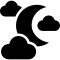
\includegraphics{./images/Nacht}

\end{column}

\begin{column}{0.04\textwidth}

~

\end{column}

\begin{column}{0.60\textwidth}

Piosenka \textbf{Nacht} \citep{Nacht} \emph{Noc} Ćwierć wieku po Het is een nacht Guus Meeuwis wykonał ``Nacht'' wraz z raperem Kraantje Pappie. Posłuchajcie sami.

\end{column}

\vfill

\begin{column}{0.48\textwidth}

\emph{Het is een nacht}\\
\emph{Die je normaal alleen in films ziet}\\
\emph{Het is een nacht}\\
\emph{Die wordt bezongen in het mooiste lied}\\
\emph{Het is een nacht}\\
\emph{Waarvan ik dacht dat ik hem nooit beleven zou}\\
\emph{Maar vannacht beleef ik hem met jou oh oh}

\end{column}

\begin{column}{0.04\textwidth}

~

\end{column}

\begin{column}{0.48\textwidth}

\emph{To jest taka noc}\\
\emph{Którą widzisz zwykle tylko w filmach}\\
\emph{To jest taka noc}\\
\emph{O której mówi najpiękniejsza piosenka}\\
\emph{To jest taka noc}\\
\emph{O której myślałem, że jej nigdy nie przeżyję}\\
\emph{A którą dziś przeżywam z tobą Ooo}

\end{column}

\vfill

\begin{column}{0.48\textwidth}

Op de grond ligt Châteauneuf-du-Pape\\
De radio zacht, rond middernacht\\
Ik hoor Suus en Freek, een blauwe dag\\
En ik kijk hoe je slaapt, ik hou je vast\\
Want ik weet dat het niet lang meer duurt voor jij gaat\\
Ik snap dat jij me niet te dichtbij laat\\
En je weer vrijmaakt en je op tijd staat\\
Je twijfelt aan of ik wel echt meen wat ik heb gezegd\\
En of ik nog steeds wel de echte ben\\
En of ik niet ren naar 050 en je niet meer ken als een slechte vent\\
Maar vannacht is dat allemaal niet de case\\
Voor nu is het nog nooit zo mooi geweest\\
Jij en ik, the road can wait\\
En ben ik voor eerst opeens compleet

\end{column}

\begin{column}{0.04\textwidth}

~

\end{column}

\begin{column}{0.48\textwidth}

Na ziemi leży Châteauneuf-du-Pape\\
Radio cicho gra, jest koło północy\\
Słyszę Suus i Freek, jakiś niebieski dzień\\
Patrzę jak śpisz, przytulam cię\\
Bo wiem, że to nie potrwa już długo zanim wyjdziesz\\
Rozumiem, że nie pozwolisz mi się zbliżyć\\
En je weer vrijmaakt en je op tijd staat\\
Wątpisz, czy naprawdę mam na myśli to, co powiedziałem\\
I czy nadal jestem prawdziwy\\
I czy nie biegnę na 50 i już cię nie znam jak jakiś zły facet\\
Ale dziś w nocy to w ogóle nie o to chodzi\\
Jeszcze nigdy nie było tak pięknie\\
Ty i ja, droga może poczekać\\
Nagle po raz pierwszy jestem spełniony

\end{column}

\vfill

\begin{column}{0.48\textwidth}

\emph{Als het komt, zou ik steeds met je zijn}\\
\emph{En als je wennen moet, begrijp ik baby, neem je de tijd}\\
\emph{Hier leven we voor, plus cash en baguettes}\\
\emph{En deze nacht heeft alles wat ik zocht op deze plek}

\end{column}

\begin{column}{0.04\textwidth}

~

\end{column}

\begin{column}{0.48\textwidth}

\emph{Gdyby tak się stało, zawsze byłbym z tobą}\\
\emph{A jeśli musisz się zastanowić, rozumiem to baby, nie spiesz się}\\
\emph{Po to żyjemy, plus kasa i bagietki}\\
\emph{I ta noc ma wszystko, co szukałem w tym miejscu}

\end{column}

\vfill

\begin{column}{0.48\textwidth}

Hey schat, ik zou m'n kleine teen geven voor nog één nacht\\
Het is natuurlijk geen wonder dat ik je\\
Donderdag al bijzonder zag in het dons gepakt heb\\
En onze nacht werd er één als\\
Die van Leo en Kate was\\
We on top of the world, ben volledig gebrainwashed\\
But I like it, yeah, jij showt wat life is\\
En ja, je life is er een als Kylie's\\
Maar net iets ronder en iets gezonder\\
Dat is precies hoe mijn vibe is, yeah\\
Jij bent de nicest\\
Bel de Bel, boy, bestel champagne\\
Fuck the prices, je rolt met Crane

\end{column}

\begin{column}{0.04\textwidth}

~

\end{column}

\begin{column}{0.48\textwidth}

Hej kochanie, oddałbym mój mały palec u nogi za jeszcze jedną noc\\
Oczywiście to nic dziwnego, że ja ciebie\\
Donderdag al bijzonder zag in het dons gepakt heb\\
A nasza noc stała się taką jedną,\\
Jaka należała do Leo i Kate\\
Jesteśmy na szczycie świata, mam kompletnie wyprany mózg\\
Ale lubię to, tak, pokazujesz, czym jest życie\\
I tak, twoje życie jest takie jak życie Kylie\\
Ale nieco bardziej zaokrąglone i nieco zdrowsze\\
Dokładnie taki jest mój klimat, tak\\
Jesteś najmilsza\\
Bel de Bel, chłopie, zamówmy szampana\\
Pieprzyć ceny, ty kręcisz z Crane

\end{column}

\vfill

\begin{column}{0.48\textwidth}

Maar vannacht beleef ik 'm met jou, oh\\
Ja ik hou alleen nog maar van jou\\
Ja ik hou alleen nog maar van jou

\end{column}

\begin{column}{0.04\textwidth}

~

\end{column}

\begin{column}{0.48\textwidth}

Ale dziś przeżywam ją z tobą Ooo\\
I kocham tylko wyłącznie ciebie\\
I kocham tylko wyłącznie ciebie

\end{column}

\vfill

\begin{quote}
\textbf{Châteauneuf-du-Pape} fr. cenione wino\\
\textbf{Suus en Freek} duet wykonujący Blauwe Dag \ref{Blauwe-dag}\\
\textbf{Leo en Kate} para z filmu Titanic\\
\textbf{Kylie} amerykańska celebrytka\\
\textbf{Bel de Bel} właść. fr. La Belle des belles\\
\textbf{Crane} od Kraantje, wykonawcy piosenki
\end{quote}

  \bibliography{songs.bib}

\end{document}
